\section{Node Coverage Guarantees Under Random Sampling}

If we draw at each evaluation step a random node and perform an action, we may ask how many evaluations are required so that we visit each of the \(\nu\) nodes at least once with high certainty.

This problem can be framed as a \emph{coupon collector's problem}~\cite{feller1968introduction}. Writing $M$ for the number of draws, the expected number of steps needed to visit all \(\nu\) nodes at least once is

\[
\mathbb{E}[M]
= \nu H_\nu
= \nu \left( \ln \nu + \gamma + O\!\left(\frac{1}{\nu}\right) \right),
\]

where \(H_\nu\) is the \(\nu\)-th harmonic number and \(\gamma \approx 0.57721\) is the Euler-Mascheroni constant.

\bigskip

Beyond the expectation, one may also ask for a high-probability guarantee.
Using the asymptotic limit for the coupon collector's completion time,
the probability that all nodes have been visited by draw

\[
M = \nu(\ln \nu + c)
\]
converges to
\[
\mathbb{P}\bigl(M \le \nu(\ln \nu + c)\bigr) \approx e^{-e^{-c}}.
\]

To achieve at least \(99\%\) probability of having visited all nodes, we solve for $c$
\[
\begin{aligned}
e^{-e^{-c}} &= p \\[8pt]
\ln\!\left(e^{-e^{-c}}\right) &= \ln(p) \\[8pt]
-e^{-c} &= \ln(p) \\[8pt]
\text{For } p = 0.99:\quad
c &= -\ln\!\bigl(-\ln(0.99)\bigr) \approx 4.60015 \approx \ln(100).
\end{aligned}
\]

Since each node is selected independently with probability $\tfrac{1}{\nu}$ at every draw,
the visit count of any particular node over $M$ draws follows a Binomial distribution,
\[
X_i \sim \mathrm{Binomial}\!\left(M, \tfrac{1}{\nu}\right),
\]
from which the expected number of visits per node is
\[
\mathbb{E}[X_i] = \frac{M}{\nu}.
\]


We evaluate four environments with differing numbers of distinct tasks and a fixed amount of draws (number of evaluations) $M=1{,}000{,}000$:

\begin{table}[h]
\centering
\caption{Coupon collector bounds for the four benchmark environments with $M=1{,}000{,}000$ total evaluations.}
\label{tab:coupon-collector}
\begin{tabular}{@{}lrrrr@{}}
\toprule
Environment & $\nu$ & $\mathbb{E}[M]$ & $M_{0.99}$ & $\mathbb{E}[X_i]$ \\
\midrule
Archery / Arm / Cartpole & 5\,000 & 45\,472 & 65\,612 & 200 \\
Hexapod              & 2\,000 & 16\,356 & 24\,412 & 500 \\
\bottomrule
\end{tabular}
\end{table}


\section{MONET Algorithm}
Algorithm~\ref{alg:individual} and Algorithm~\ref{alg:social} detail the two learning subroutines invoked in Algorithm~\ref{alg:monet}.

\paragraph{Individual Learning.}
When individual learning is selected, the current elite at node $\boldsymbol{\tau}_i$ is mutated independently of any neighbor. If no solution exists at the node, a random solution is drawn from $\mathcal{U}(p_{\min}, p_{\max})$ and evaluated. Otherwise, Gaussian mutation with standard deviation $\sigma_m$ scaled by the parameter range is applied. The offspring replaces the current elite only if its fitness is at least as high.

\begin{algorithm}[H]
\caption{Individual Learning}\label{alg:individual}
\begin{algorithmic}[1]
\Require Task $\boldsymbol{\tau}$, archive $\mathcal{A}$, bounds $p_{\min}, p_{\max}$, mutation std $\sigma_m$
\Ensure Updated $\mathcal{A}[\boldsymbol{\tau}]$
\If{$\mathcal{A}[\boldsymbol{\tau}] = \emptyset$} \Comment{initialize empty node}
    \State $\boldsymbol{\theta} \sim \mathcal{U}(p_{\min}, p_{\max})$ \Comment{random solution}
    \State $\mathcal{A}[\boldsymbol{\tau}] \gets (\boldsymbol{\theta},\, f(\boldsymbol{\theta}, \boldsymbol{\tau}))$
    \State \Return
\EndIf
\State $\boldsymbol{\theta} \gets \mathcal{A}[\boldsymbol{\tau}].\text{solution}$ \Comment{current elite}
\State $\boldsymbol{\epsilon} \sim \mathcal{N}(\mathbf{0},\, \sigma_m (p_{\max} - p_{\min}))$ \Comment{Gaussian perturbation}
\State $\mathbf{y} \gets \text{clip}(\boldsymbol{\theta} + \boldsymbol{\epsilon},\; p_{\min},\; p_{\max})$ \Comment{mutant offspring}
\State $f_y \gets f(\mathbf{y}, \boldsymbol{\tau})$
\If{$f_y \geq \mathcal{A}[\boldsymbol{\tau}].\text{fitness}$} \Comment{elitist replacement}
    \State $\mathcal{A}[\boldsymbol{\tau}] \gets (\mathbf{y}, f_y)$
\EndIf
\end{algorithmic}
\end{algorithm}

\paragraph{Social Learning.}
When social learning is selected, the current elite is recombined with a solution drawn from a neighboring node. If the current node is empty, the neighbor's solution is copied as an initial seed (or a random solution is used when no neighbor has a solution). Recombination is performed via Simulated Binary Crossover (SBX)~\cite{SBX} with distribution index $\eta_c=10$~\cite{deb2001multi}. As with individual learning, the offspring replaces the elite only upon improvement.

\begin{algorithm}[H]
\caption{Social Learning}\label{alg:social}
\begin{algorithmic}[1]
\Require Task $\boldsymbol{\tau}$, neighbor task $\boldsymbol{\tau}_j$, archive $\mathcal{A}$, bounds $p_{\min}, p_{\max}$
\Ensure Updated $\mathcal{A}[\boldsymbol{\tau}]$
\If{$\mathcal{A}[\boldsymbol{\tau}] = \emptyset$} \Comment{initialize empty node}
    \If{$\mathcal{A}[\boldsymbol{\tau}_j] \neq \emptyset$}
        \State $\boldsymbol{\theta} \gets \mathcal{A}[\boldsymbol{\tau}_j].\text{solution}$ \Comment{copy from neighbor}
    \Else
        \State $\boldsymbol{\theta} \sim \mathcal{U}(p_{\min}, p_{\max})$ \Comment{random fallback}
    \EndIf
    \State $\mathcal{A}[\boldsymbol{\tau}] \gets (\boldsymbol{\theta},\, f(\boldsymbol{\theta}, \boldsymbol{\tau}))$
    \State \Return
\EndIf
\If{$\mathcal{A}[\boldsymbol{\tau}_j] = \emptyset$}
    \State \Return \Comment{no valid neighbor solution}
\EndIf
\State $\mathbf{y} \gets \text{SBX}\bigl(\mathcal{A}[\boldsymbol{\tau}].\text{solution},\; \mathcal{A}[\boldsymbol{\tau}_j].\text{solution},\; \eta_c\!=\!10\bigr)$ \Comment{crossover}
\State $\mathbf{y} \gets \text{clip}(\mathbf{y},\, p_{\min},\, p_{\max})$
\State $f_y \gets f(\mathbf{y}, \boldsymbol{\tau})$
\If{$f_y \geq \mathcal{A}[\boldsymbol{\tau}].\text{fitness}$} \Comment{elitist replacement}
    \State $\mathcal{A}[\boldsymbol{\tau}] \gets (\mathbf{y}, f_y)$
\EndIf
\end{algorithmic}
\end{algorithm}

\section{Closed-Form Task Fitness Definitions}\label{app:tasks}

This appendix gives the explicit fitness expressions for the four benchmarks.

\subsection{Archery}
With initial velocity vector
\[
\mathbf{v} = v_0
\begin{bmatrix}
-\sin(\text{yaw}) \\
\cos(\text{yaw})\cos(\text{pitch}) \\
\cos(\text{yaw})\sin(\text{pitch})
\end{bmatrix},
\quad v_0 = 70\,\mathrm{m/s},
\]
the target-plane hit time is $t_{\text{hit}} = D/v_y$ whenever $v_y > 0$; if $v_y \le 0$ the shot misses and $f = 0$. Taking $g = 9.8\,\mathrm{m/s^2}$ and wind $W\in[-10,10]\,\mathrm{m/s^2}$ along $x$, the miss coordinates on the target plane ($y = D$) are
\[
m_x = \tfrac{1}{2}\,W\,t_{\text{hit}}^2 + v_x\,t_{\text{hit}},
\qquad
m_z = -\tfrac{1}{2}\,g\,t_{\text{hit}}^2 + v_z\,t_{\text{hit}},
\qquad
r = \sqrt{m_x^2 + m_z^2}.
\]
Fitness is computed on a 10-ring target of ring width $0.061\,\mathrm{m}$:
\[
f = \frac{\max\!\bigl(0,\; 10 - \lfloor r/0.061 \rfloor\bigr)}{10} \in \{0, 0.1, \ldots, 1.0\}.
\]

\subsection{Arm}
With end-effector position $\mathbf{p}_{\text{ee}}\in\mathbb{R}^2$ and a fixed target $\mathbf{p}_{\text{tar}} = (0.5, 0.5)$,
\[
f = \exp\!\left(-\lVert \mathbf{p}_{\text{ee}} - \mathbf{p}_{\text{tar}} \rVert_2\right) \in (0,1].
\]
The joint commands are $\mathbf{q} = (\boldsymbol{\theta}-\tfrac{1}{2})\cdot 2\pi\,\alpha_{\max}/10$ where $\boldsymbol{\theta}\in[0,1]^{10}$ is the solution vector and $\alpha_{\max}$ is the task-dependent maximum joint-angle fraction; each of the $10$ links has length $L/10$ with $L$ the task-dependent total arm length. $\mathbf{p}_{\text{ee}}$ is the end-effector position returned by forward kinematics.

\subsection{Cartpole}
The task uses the \texttt{CartPole-v1} dynamics from OpenAI Gym with the pole mass $m_p$ and pole length $L$ replaced by the per-task values; the default cart mass $m_c$ is retained. With pole angle $\phi$, cart position $x_c$, control force $F\in\{-10, +10\}\,\mathrm{N}$, and gravity $g=9.8\,\mathrm{m/s^2}$,
\[
\ddot{\phi} = \frac{g \sin \phi + \cos \phi \left(-F - m_p L \dot{\phi}^2 \sin \phi\right)/(m_c + m_p)}{L \left(\tfrac{4}{3} - \tfrac{m_p \cos^2 \phi}{m_c + m_p}\right)},
\qquad
\ddot{x}_c = \frac{F + m_p L \left(\dot{\phi}^2 \sin \phi - \ddot{\phi} \cos \phi\right)}{m_c + m_p}.
\]
A solution is evaluated over $n_{\text{rollouts}} = 10$ rollouts with distinct Gym seeds. Each rollout runs until the pole leaves the balanced region ($|\phi| \ge 12^\circ$ or $|x_c| \ge 2.4\,\mathrm{m}$) or until the step cap $t_{\max}=1000$ is reached. Writing $t_{\text{balanced}}^{(k)}$ for the number of surviving steps on rollout $k$, the reported fitness is the arithmetic mean
\[
f = \frac{1}{n_{\text{rollouts}}}\sum_{k=1}^{n_{\text{rollouts}}} \min\!\bigl(t_{\max},\, t_{\text{balanced}}^{(k)}\bigr) \in [0, t_{\max}].
\]

\subsection{Hexapod}
With gait parameters $\boldsymbol{\theta}\in[0,1]^{36}$ and morphology $\boldsymbol{\tau}\in\mathcal{T}$ instantiated through a per-task URDF, a PyBullet simulation is run for up to $3\,\mathrm{s}$ of wall-clock simulator time. The episode terminates early if any body-axis angle (roll, pitch, yaw) exceeds $\pi/8$ or if the lateral deviation satisfies $|y|>0.5\,\mathrm{m}$. Writing $p_x(t)$ for the forward position of the center of mass and $T\le 3\,\mathrm{s}$ for the time of termination or episode end,
\[
f(\boldsymbol{\theta},\boldsymbol{\tau}) = p_x(T),
\]
reported in metres. The controller returns $f=0$ if any entry of $\boldsymbol{\theta}$ lies outside $[0,1]$.


\section{Detailed Sensitivity Analysis}\label{app:sensitivity}

This appendix provides per-domain SHAP beeswarm plots and the SPOT-tuned hyperparameter configurations that complement the global sensitivity analysis.

\subsection{Per-Domain SHAP Analysis}

Figures~\ref{fig:shap-archery} and~\ref{fig:shap-arm} show the SHAP beeswarm plots for the archery and arm domains, respectively. Each point represents one MONET run; its horizontal position indicates the SHAP value (contribution to the predicted metric), and its color encodes the feature value (red = high, blue = low).

In both domains, $p_\text{ind}$ exhibits the strongest effect: high values of $p_\text{ind}$ (more individual learning) consistently decrease predicted fitness, corroborating the global finding that social learning is the primary driver of performance. The remaining parameters show smaller, more task-specific effects.

\begin{figure}[H]
    \centering
    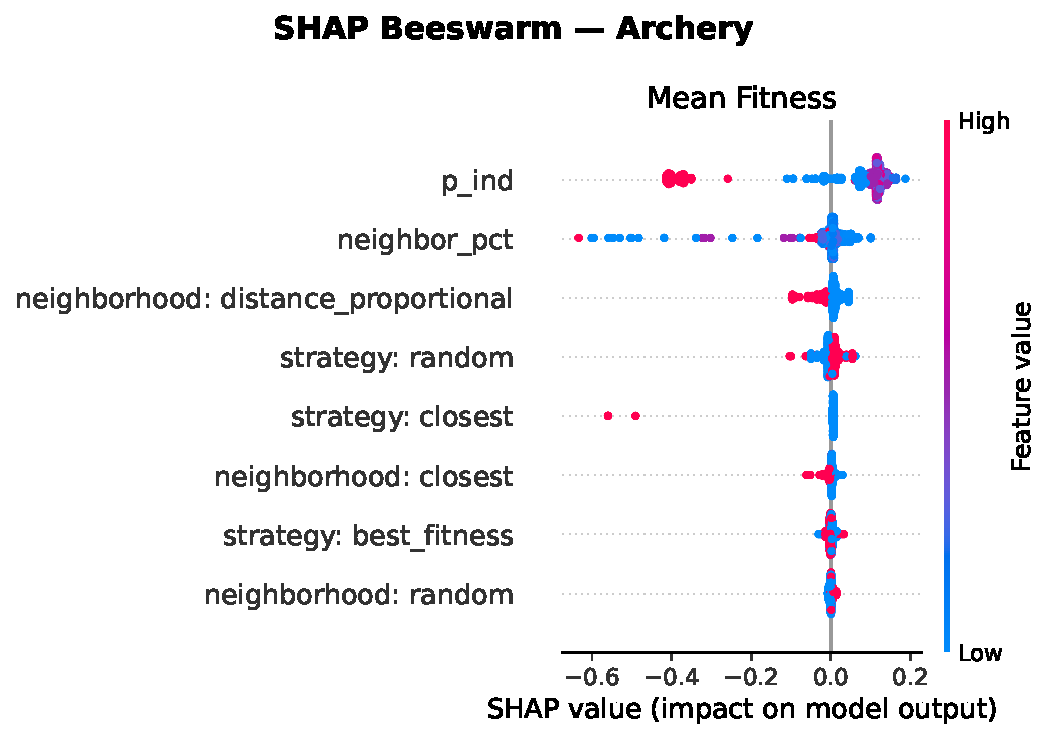
\includegraphics[width=1\linewidth]{figs/monet_hyperparam_importance_archery.pdf}
    \caption{SHAP beeswarm plot for the archery domain. Each row is a hyperparameter; each dot is a MONET run. Color indicates the feature value (red = high, blue = low); horizontal position indicates the SHAP value.}
    \label{fig:shap-archery}
\end{figure}

\begin{figure}[H]
    \centering
    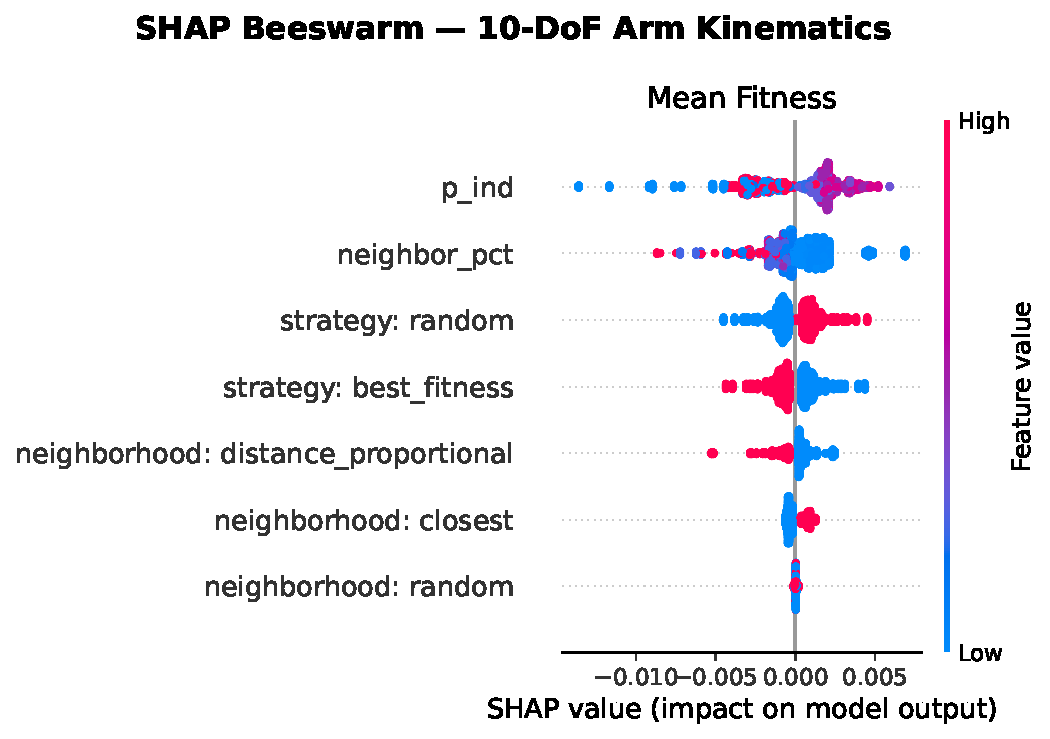
\includegraphics[width=1\linewidth]{figs/monet_hyperparam_importance_arm.pdf}
    \caption{SHAP beeswarm plot for the arm domain. Panels as in Figure~\ref{fig:shap-archery}.}
    \label{fig:shap-arm}
\end{figure}

\begin{figure}[H]
    \centering
    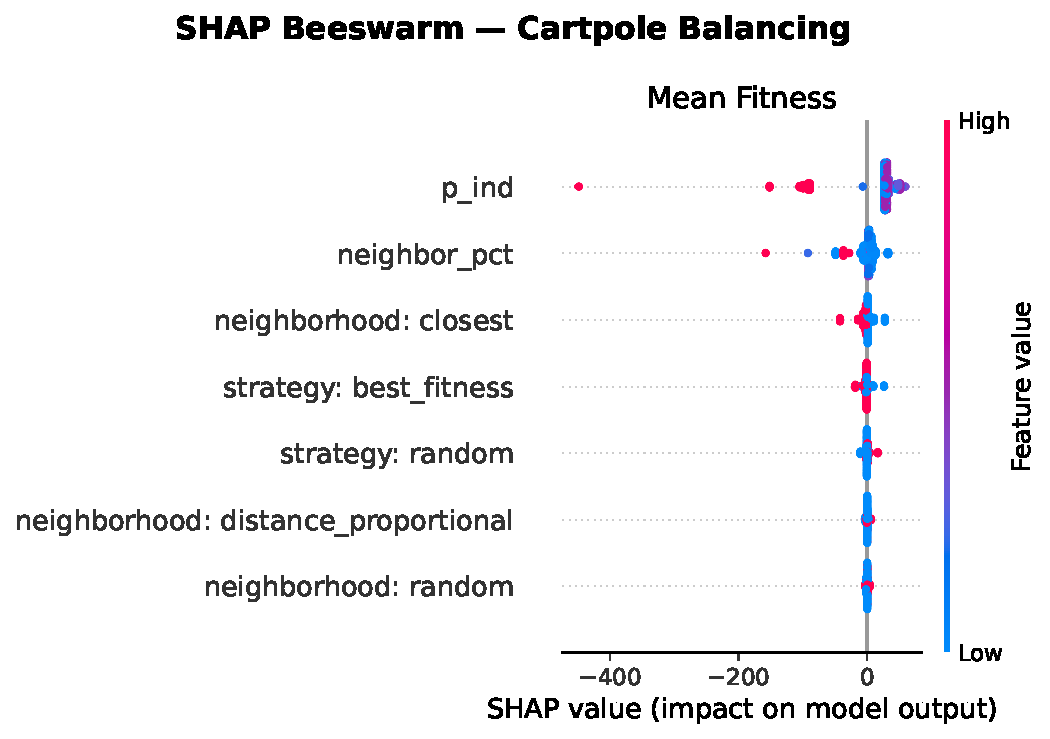
\includegraphics[width=1\linewidth]{figs/monet_hyperparam_importance_cartpole.pdf}
    \caption{SHAP beeswarm plot for the cartpole domain. Panels as in Figure~\ref{fig:shap-archery}.}
    \label{fig:shap-cartpole}
\end{figure}

\begin{figure}[H]
    \centering
    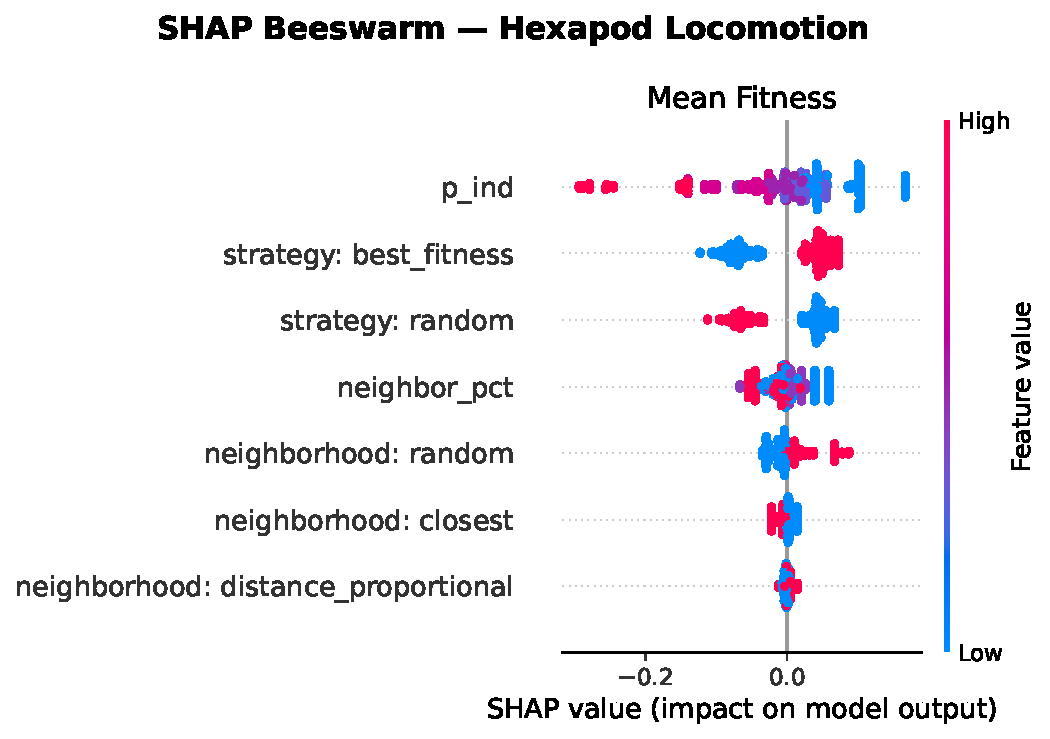
\includegraphics[width=1\linewidth]{figs/monet_hyperparam_importance_hexapod.pdf}
    \caption{SHAP beeswarm plot for the hexapod domain. Panels as in Figure~\ref{fig:shap-archery}.}
    \label{fig:shap-hexapod}
\end{figure}

\subsection{SPOT-Tuned Configurations}

Table~\ref{tab:spot-configs} lists the per-domain configurations found by the SPOT hyperparameter tuner.

\begin{table}[h]
\centering
\caption{SPOT-tuned MONET configurations per domain.}
\label{tab:spot-configs}
\small
\begin{tabular}{@{}lllcc@{}}
\toprule
\textbf{Domain} & \textbf{strategy} & \textbf{neighborhood} & $p_\text{ind}$ & \textbf{neighbor\_pct.} \\
\midrule
Archery  & best\_fitness & closest  & 0.0 & 2\% \\
Arm      & random        & closest  & 0.3 & 1\% \\
Cartpole & best\_fitness & random   & 0.5 & 1\% \\
Hexapod  & best\_fitness & random   & 0.0 & 1\% \\
\bottomrule
\end{tabular}
\end{table}

\section{MONET Hyperparameter Descriptions}\label{app:hyperparameters}

Table~\ref{tab:monet-hyperparams} summarizes the four hyperparameters varied in the sensitivity analysis. All other algorithmic parameters (mutation operator, crossover operator, initialization strategy) are held fixed throughout. See Algorithm~\ref{alg:monet} for the points at which each parameter enters the loop.

\begin{table}[h]
\centering
\caption{MONET hyperparameters and their roles.}
\label{tab:monet-hyperparams}
\renewcommand{\arraystretch}{1.3}
\small
\begin{tabular}{@{}p{2.4cm}p{2.2cm}p{7.4cm}@{}}
\toprule
\textbf{Parameter} & \textbf{Values} & \textbf{Description} \\
\midrule
$p_\text{ind}$ &
0, 0.3, 0.5, 0.7, 1 &
Probability that a given evaluation step performs \emph{individual learning} (mutation of the focal task's own elite) rather than \emph{social learning} (crossover with a neighbor's elite). At $p_\text{ind}=0$ only social learning occurs; at $p_\text{ind}=1$ only individual learning occurs. \\
\addlinespace
strategy &
random, best\_fitness &
Neighbor selection strategy during social learning. \texttt{random}: uniform random selection among all neighbors. \texttt{best\_fitness}: deterministically select the neighbor with the highest current fitness. \\
\addlinespace
neighborhood &
random, closest, distance\_prop. &
Method for constructing the neighbor set of each task.
\texttt{closest}: the $N$ nearest tasks by Euclidean distance in task space.
\texttt{random}: $N$ tasks sampled uniformly at random (sorted by similarity after sampling).
\texttt{distance\_proportional}: $N$ tasks sampled \emph{without replacement} with probability proportional to task-space similarity $s(\boldsymbol{\tau}_i, \boldsymbol{\tau}_j) = 1/(1 + \lVert \boldsymbol{\tau}_i - \boldsymbol{\tau}_j \rVert)$; this softly biases the neighborhood toward nearby tasks while retaining a chance of including distant ones. \\
\addlinespace
neighbor\_pct. &
1\%, 5\%, 10\% &
Fraction of the total task set used as the neighborhood size~$N = \lceil \texttt{neighbor\_percentage} \cdot |\mathcal{V}| \rceil$. For instance, with 5\,000 tasks and 5\%, each task has $N=250$ neighbors. Controls graph sparsity: lower values yield sparser graphs with more localized knowledge transfer. \\
\bottomrule
\end{tabular}
\end{table}


\section{Hyperparameter Configuration Ranking}\label{app:ranking}

Table~\ref{tab:top10} lists the ten highest-ranked MONET hyperparameter configurations (across the 2--4 domains on which they were run) by combined z-score, computed as the mean of the within-domain z-scores of final mean fitness and AUC. Table~\ref{tab:bottom5} shows the five worst-ranked configurations for comparison. Only configurations evaluated on at least two domains are included in the ranking. The counts $n_{\text{Arm}}, n_{\text{Archery}}, n_{\text{Cartpole}}, n_{\text{Hexapod}}$ report the number of deduplicated seed runs per domain.

\begin{table}[h]
\centering
\caption{Top 10 MONET configurations by combined z-score ($n_{\text{domains}} \ge 2$).}
\label{tab:top10}
\footnotesize
\setlength{\tabcolsep}{3pt}
\begin{tabular}{@{}llrrrrrrrrr@{}}
\toprule
strategy & neighborhood & nbr.\% & $p_\text{ind}$ & $n_\text{Arm}$ & $n_\text{Arc}$ & $n_\text{Cart}$ & $n_\text{Hex}$ & $z_{\text{FF}}$ & $z_{\text{AUC}}$ & combined \\
\midrule
best\_fitness & closest               & 1.5 & 0.30 & 20 & 20 &  0 &  0 & $+0.58$ & $+1.01$ & $\mathbf{+0.80}$ \\
best\_fitness & closest               & 1.0 & 0.30 & 22 & 22 &  0 &  5 & $+0.60$ & $+0.96$ & $+0.78$ \\
best\_fitness & closest               & 2.0 & 0.30 & 20 & 20 &  0 &  0 & $+0.55$ & $+0.99$ & $+0.77$ \\
best\_fitness & closest               & 2.0 & 0.50 & 20 & 39 &  5 &  0 & $+0.62$ & $+0.90$ & $+0.76$ \\
best\_fitness & closest               & 1.5 & 0.70 &  5 & 20 &  0 &  0 & $+0.62$ & $+0.81$ & $+0.72$ \\
best\_fitness & closest               & 2.0 & 0.70 &  5 & 20 &  0 &  0 & $+0.62$ & $+0.82$ & $+0.72$ \\
random        & closest               & 2.0 & 0.00 & 20 & 19 &  4 &  0 & $+0.66$ & $+0.75$ & $+0.71$ \\
random        & closest               & 1.5 & 0.00 & 20 & 19 &  5 &  0 & $+0.66$ & $+0.75$ & $+0.70$ \\
best\_fitness & closest               & 1.0 & 0.50 & 40 & 41 &  5 &  5 & $+0.56$ & $+0.82$ & $+0.69$ \\
random        & closest               & 1.0 & 0.00 & 40 & 40 &  5 &  3 & $+0.64$ & $+0.73$ & $+0.68$ \\
\bottomrule
\end{tabular}
\end{table}

\begin{table}[h]
\centering
\caption{Bottom 5 MONET configurations by combined z-score ($n_{\text{domains}} \ge 2$).}
\label{tab:bottom5}
\footnotesize
\setlength{\tabcolsep}{3pt}
\begin{tabular}{@{}llrrrrrrrrr@{}}
\toprule
strategy & neighborhood & nbr.\% & $p_\text{ind}$ & $n_\text{Arm}$ & $n_\text{Arc}$ & $n_\text{Cart}$ & $n_\text{Hex}$ & $z_{\text{FF}}$ & $z_{\text{AUC}}$ & combined \\
\midrule
best\_fitness & distance\_prop.\       &  5.0 & 1.00 & 20 & 20 &  0 &  2 & $-1.22$ & $-1.86$ & $-1.54$ \\
best\_fitness & distance\_prop.\       & 10.0 & 0.00 & 20 & 20 &  0 & 16 & $-2.51$ & $-0.65$ & $-1.58$ \\
random        & closest               & 34.3 & 0.98 &  2 &  1 &  1 &  0 & $-1.19$ & $-1.97$ & $-1.58$ \\
best\_fitness & distance\_prop.\       &  5.0 & 0.00 & 20 & 20 &  0 &  3 & $-3.00$ & $-0.93$ & $-1.96$ \\
best\_fitness & distance\_prop.\       & 41.5 & 0.99 &  2 &  2 &  2 &  0 & $-1.97$ & $-2.23$ & $\mathbf{-2.10}$ \\
\bottomrule
\end{tabular}
\end{table}

Two patterns are clear from Table~\ref{tab:top10}: (i)~the \texttt{closest} neighborhood dominates the top of the ranking, and (ii)~small neighborhood sizes ($\le 2\%$ of the task set) are preferred. Poorly-performing configurations (Table~\ref{tab:bottom5}) combine the \texttt{distance\_proportional} neighborhood with either very high $p_\text{ind}$ (near pure individual learning) or very large neighborhoods, both of which disrupt local knowledge transfer.

\section{Code Availability}\label{app:code}

Table~\ref{tab:code-availability} lists the reference papers and public code repositories for MONET and the three baselines.

\begin{table}[h]
\centering
\caption{Reference papers and public code repositories for MONET and the baseline algorithms.}
\label{tab:code-availability}
\small
\setlength{\tabcolsep}{4pt}
\begin{tabular}{@{}lll@{}}
\toprule
\textbf{Algorithm} & \textbf{Paper} & \textbf{Code} \\
\midrule
MONET (ours) & This paper                                                    & \cite{monet_code} \\
MAP-Elites   & \cite{DBLP:journals/corr/MouretC15,MAP_Elites_NaturePaper}    & \cite{pymap_elites_code} \\
MT-ME        & \cite{mouretQualitydiversitymultitaskoptimization2020}        & \cite{pymap_elites_code} \\
PT-ME        & \cite{anneParametricTaskMAPElites2024}                        & \cite{pt_me_code} \\
\bottomrule
\end{tabular}
\end{table}